\documentclass[conference, a4paper]{IEEEtran}[2015/08/26]
\IEEEoverridecommandlockouts
% Template version as of 6/27/2024

\usepackage{cite}
\usepackage{amsmath,amssymb,amsfonts}
\usepackage{algorithmic}
\usepackage{graphicx}
\usepackage{textcomp}
\usepackage{xcolor}
\usepackage{float}
\usepackage{placeins}
\usepackage{colortbl}
\usepackage{xcolor}
\usepackage[square,comma,numbers,sort&compress]{natbib}
\renewcommand{\bibfont}{\normalfont\footnotesize}
\usepackage{balance}

\def\BibTeX{{\rm B\kern-.05em{\sc i\kern-.025em b}\kern-.08em
    T\kern-.1667em\lower.7ex\hbox{E}\kern-.125emX}}
\begin{document}

\title{EXTENDED RTAB-Map AND REDUCED Fast-SCNN FOR AUTONOMOUS INDUSTRIAL VEHICLE NAVIGATION}

\author{\IEEEauthorblockN{Azzam Wildan Maulana}
\IEEEauthorblockA{\textit{Department of Electrical Engineering} \\
Institut Teknologi Sepuluh Nopember\\
Surabaya, Indonesia 60111 \\
6022241101@student.its.ac.id}
\and
\IEEEauthorblockN{Rudy Dikairono}
\IEEEauthorblockA{\textit{Department of Electrical Engineering}\\
Institut Teknologi Sepuluh Nopember\\
Surabaya, Indonesia 60111 \\
rudydikairono@its.ac.id}
\and
\IEEEauthorblockN{Ahmad Zaini}
\IEEEauthorblockA{\textit{Department of Electrical and Computer Engineering}\\
Institut Teknologi Sepuluh Nopember\\
Surabaya, Indonesia 60111 \\
zaini@its.ac.id}
\and
\IEEEauthorblockN{Mauridhi Hery Purnomo}
\IEEEauthorblockA{\textit{Department of Electrical and Computer Engineering}\\
Institut Teknologi Sepuluh Nopember\\
Surabaya, Indonesia 60111 \\
hery@ee.its.ac.id}
\and
\IEEEauthorblockN{Moh Ismarintan Zazuli}
\IEEEauthorblockA{\textit{Department of Electrical Automation Engineering} \\
Institut Teknologi Sepuluh Nopember\\
Surabaya, Indonesia 60111 \\
ismarintan@its.ac.id}
\and
\IEEEauthorblockN{Muhtadin}
\IEEEauthorblockA{\textit{Department of Computer Engineering} \\
Institut Teknologi Sepuluh Nopember\\
Surabaya, Indonesia 60111 \\
muhtadin@ee.its.ac.id}
}

\maketitle

\begin{abstract}
This research develops a dual-layer navigation system for industrial autonomous vehicles. The first layer, an Extended RTAB-Map, performs global navigation and mapping; the second, a Reduced Fast-SCNN, handles local perception for lane detection. The Extended RTAB-Map introduces a skip connection from hardware odometry to pose fusion. The Reduced Fast-SCNN decreases convolutional channels and replaces pyramid pooling with average pooling. Experiments show an increase in pose update rate from 1~Hz to 50~Hz with centimeter-level accuracy (error $<5$~cm). The Reduced Fast-SCNN achieves real-time CPU-only inference below 10~ms.
\end{abstract}

\begin{IEEEkeywords}
autonomous vehicle, navigation system, machine learning, graph-based SLAM, lane detection
\end{IEEEkeywords}

\section{Introduction}
Autonomous vehicles are increasingly vital in industrial logistics, offering improvements in safety, efficiency, and operational precision. Industrial plants often require continuous material transport in constrained and hazardous environments, where human operators are prone to fatigue and error. As reported in \cite{ref_sleep}, night-shift workers are particularly susceptible to micro-sleep episodes lasting 1--2 seconds, which can result in serious accidents. To mitigate these risks, autonomous vehicles can replace or assist human-operated systems, ensuring continuous and safe material handling.

\par
An autonomous navigation system generally consists of two main components: the global navigation system for pose estimation and mapping, and the local navigation system for short-range perception and motion control. The global system requires both accuracy and high update rates to maintain stable control. In this study, we extend the Real-Time Appearance-Based Mapping (RTAB-Map) algorithm \cite{ref_rtabmap}, a graph-based SLAM framework known for its robustness in visual and LiDAR mapping. However, the default RTAB-Map provides a limited update rate (around 1~Hz) and is heavily dependent on visual odometry, which suffers under lighting variations or occlusions \cite{ref_vslam}. To overcome these limitations, an \textit{Extended RTAB-Map} is proposed by introducing a skip connection from hardware odometry to pose fusion. Odometry data from encoders and IMU sensors are combined with RTAB-Map’s corrected pose using a Kalman Filter \cite{ref_mas_marin}, improving both update frequency and pose accuracy.

\par
For local navigation, lane or drivable-area detection is essential for maintaining safe motion. Deep learning-based semantic segmentation models like Fast-SCNN \cite{ref_fast_scnn} are efficient but still computationally heavy for CPU-only systems. Although D-Fast-SCNN \cite{ref_dfast_scnn} improves accuracy using dilation, it increases inference time. To meet real-time industrial demands, we design a \textit{Reduced Fast-SCNN} by lowering convolutional channels and replacing pyramid pooling with average pooling, achieving sub-10~ms inference on CPU. The output segmentation provides a confidence level used to adjust vehicle speed and steering dynamically. By integrating the Extended RTAB-Map and Reduced Fast-SCNN, this research delivers a high-frequency, CPU-efficient, and centimeter-accurate navigation system suitable for industrial autonomous vehicles.

\section{Methodology}
The methodology of this research is divided into three main parts. The first part discusses the architecture of the Extended RTAB-Map. The second part presents the network design of the Reduced Fast-SCNN. The final part explains the integration of the Extended RTAB-Map and Reduced Fast-SCNN into a unified navigation system for autonomous industrial vehicles.

\subsection{Extended RTAB-Map for Global Navigation System}
\begin{figure}[H]
	\centering
	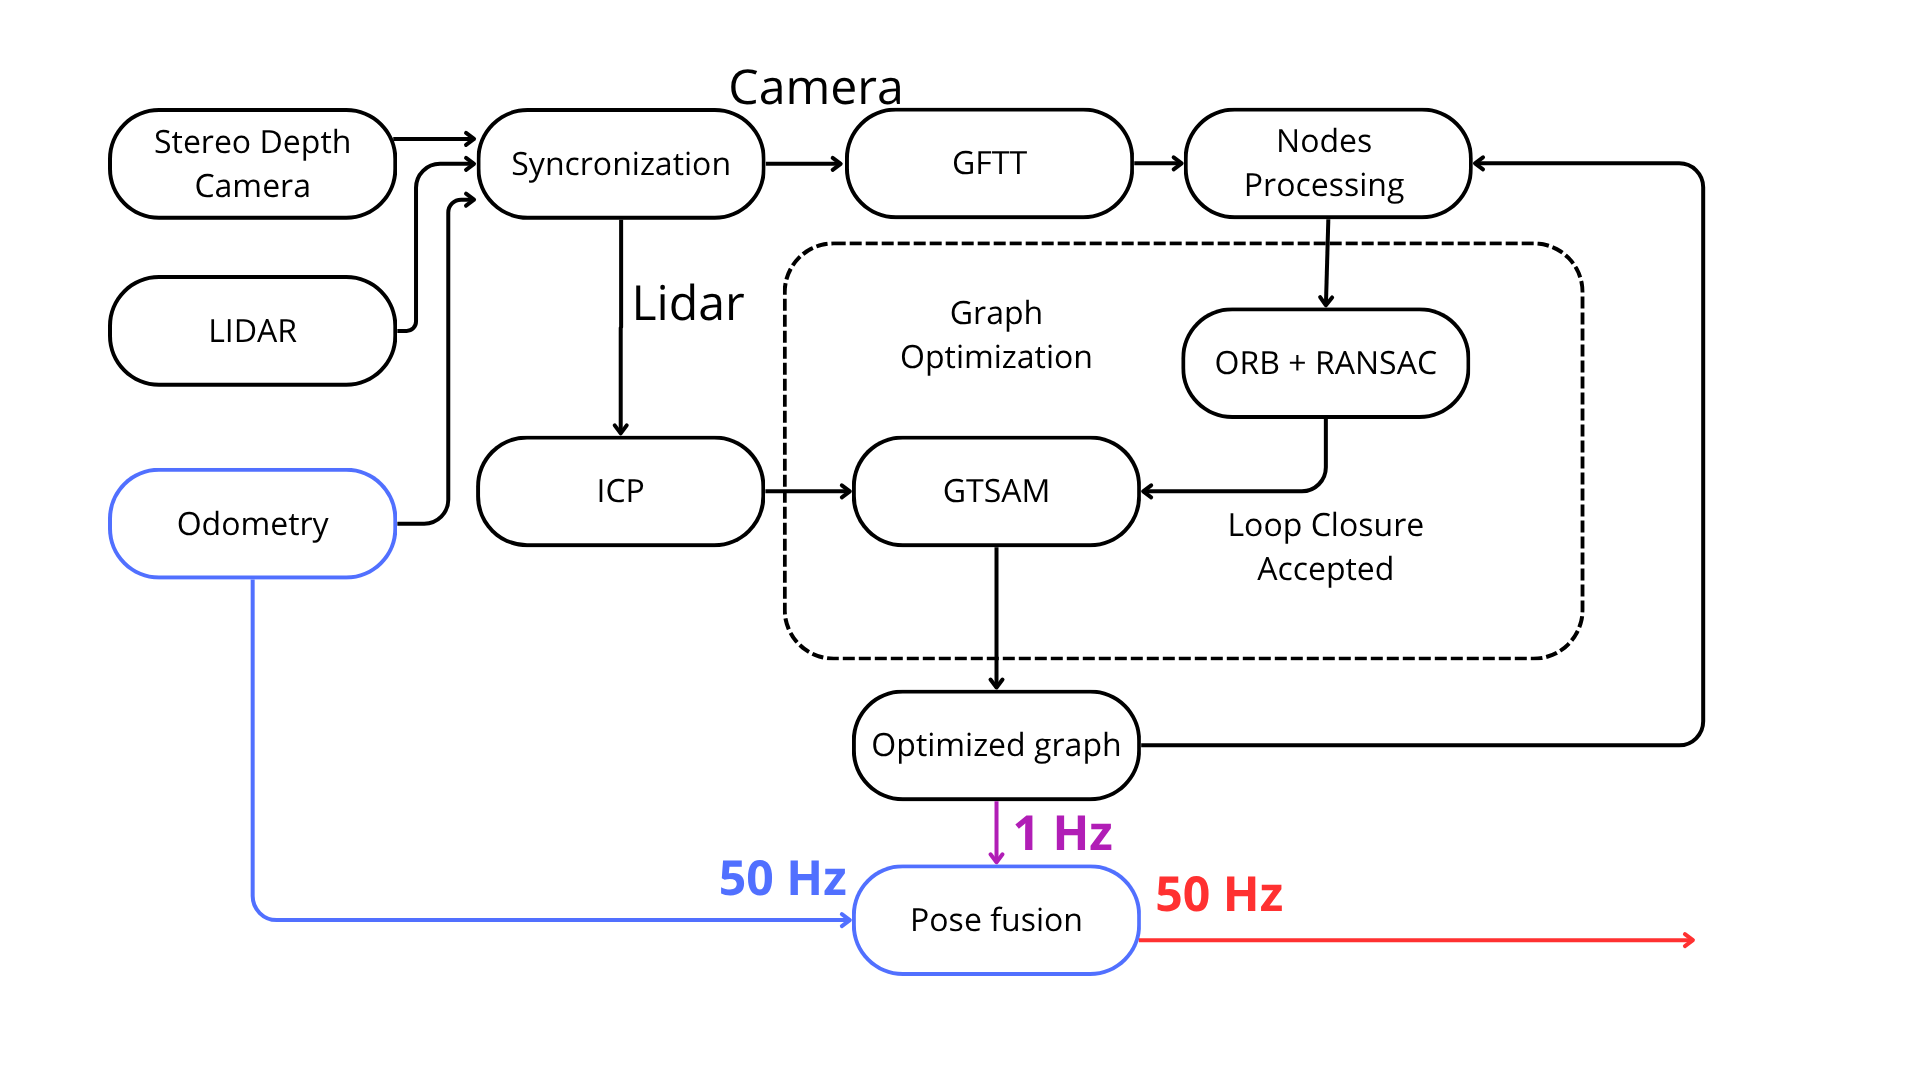
\includegraphics[width=\linewidth]{../konten/slam_fix_iki.png}
	\caption{Block diagram of graph-based SLAM in mapping mode.}
	\label{fig:slam_system}
\end{figure}

The first and most important step is to calculate the hardware odometry using encoder speed and IMU data. The relationship can be expressed as follows:

\begin{equation}
	\begin{bmatrix}
	v_x \\
	v_y \\
	v_\theta
	\end{bmatrix}
	=
	\dfrac{1}{\Delta t}
	\begin{bmatrix}
	\text{encoder\_to\_meter}\,\text{encoder\_speed}\,\cos\theta \\
	\text{encoder\_to\_meter}\,\text{encoder\_speed}\,\sin\theta \\
	\text{current\_IMUyaw}-\text{previous\_IMUyaw}
	\end{bmatrix}
	\label{eq:velocity_matrix_explicit}
\end{equation}

Here, $v_x$ represents the linear velocity in the x-direction, $v_y$ is the linear velocity in the y-direction, and $v_\theta$ is the angular velocity around the z-axis. The term $\Delta t$ denotes the time difference between the current and previous readings (20~ms). The variable $\text{encoder\_to\_meter}$ is a conversion factor from encoder speed (in rpm) to meters per second. $\text{encoder\_speed}$ refers to the encoder output, $\theta$ is the yaw angle from the IMU in radians, while $\text{current\_IMUyaw}$ and $\text{previous\_IMUyaw}$ denote the consecutive IMU yaw readings in degrees.

\par
The second step is to utilize and optimize the RTAB-Map framework. The first enhancement involves performing approximate time synchronization among camera, LiDAR, and hardware odometry data. This step is essential because each sensor operates at a different update frequency, and desynchronized data could lead to mapping errors.

\par
The second optimization of RTAB-Map involves the use of the GFTT (Good Features to Track) algorithm as an image feature detector. As demonstrated in \cite{ref_image_matching}, GFTT provides a fast yet reliable feature extraction performance suitable for real-time applications. The third improvement applies the combination of ORB (Oriented FAST and Rotated BRIEF) and RANSAC (Random Sample Consensus) for feature matching. ORB provides a computationally efficient descriptor while maintaining robustness, and RANSAC filters out outliers from matched keypoints \cite{ref_orb_ransac}. The output of this step is a loop-closure hypothesis, which indicates that the robot has revisited a previously mapped location. This hypothesis is used to refine and optimize the pose graph.

\par
The fourth enhancement in RTAB-Map involves applying the ICP (Iterative Closest Point) algorithm to establish constraints between the nodes. ICP is utilized to compute the relative pose and covariance between two adjacent nodes \cite{ref_icp}. This algorithm is selected because LiDAR laser scans provide higher geometric accuracy compared to depth information from cameras.

\par
The fifth stage involves full graph optimization using all nodes and edges. When a valid loop-closure hypothesis is detected, the corrected pose and covariance are calculated based on the ICP constraint. These values are then used to optimize the entire pose graph through nonlinear optimization using the GTSAM library \cite{ref_gtsam}. This optimization reduces accumulated drift and improves global map consistency.

\par
Despite these improvements, the standard RTAB-Map implementation yields an average pose update rate of only 1~Hz when tested on an Intel i5 12th Gen processor with 16~GB of RAM and no dedicated GPU. To increase the update rate, we introduce a skip connection from the hardware odometry to the pose fusion module (indicated by the blue line in Fig.~\ref{fig:slam_system}). The pose fusion employs a Kalman Filter to combine the corrected pose and covariance from RTAB-Map with the odometry-based pose and covariance from the hardware sensors. The hardware odometry, calculated from Eq.~\ref{eq:velocity_matrix_explicit}, serves as the velocity model in the Kalman Filter, while the RTAB-Map output acts as the measurement model.

\par
The fusion strategy begins by assigning a low covariance value (around 0.01) to the hardware odometry, prioritizing responsiveness during the vehicle’s initial motion. As the system detects more loop closures, the covariance of the RTAB-Map corrected pose gradually decreases, allowing it to dominate the fusion process. Consequently, the final pose estimation becomes both accurate and smooth over time. The use of the Kalman Filter not only improves pose accuracy but also minimizes abrupt transitions during map corrections. The resulting fused pose achieves a 50~Hz update rate on the same hardware setup, with centimeter-level precision suitable for real-time navigation.

\subsection{Reduced Fast-SCNN for Local Navigation System}
\begin{figure}[H]
	\centering
	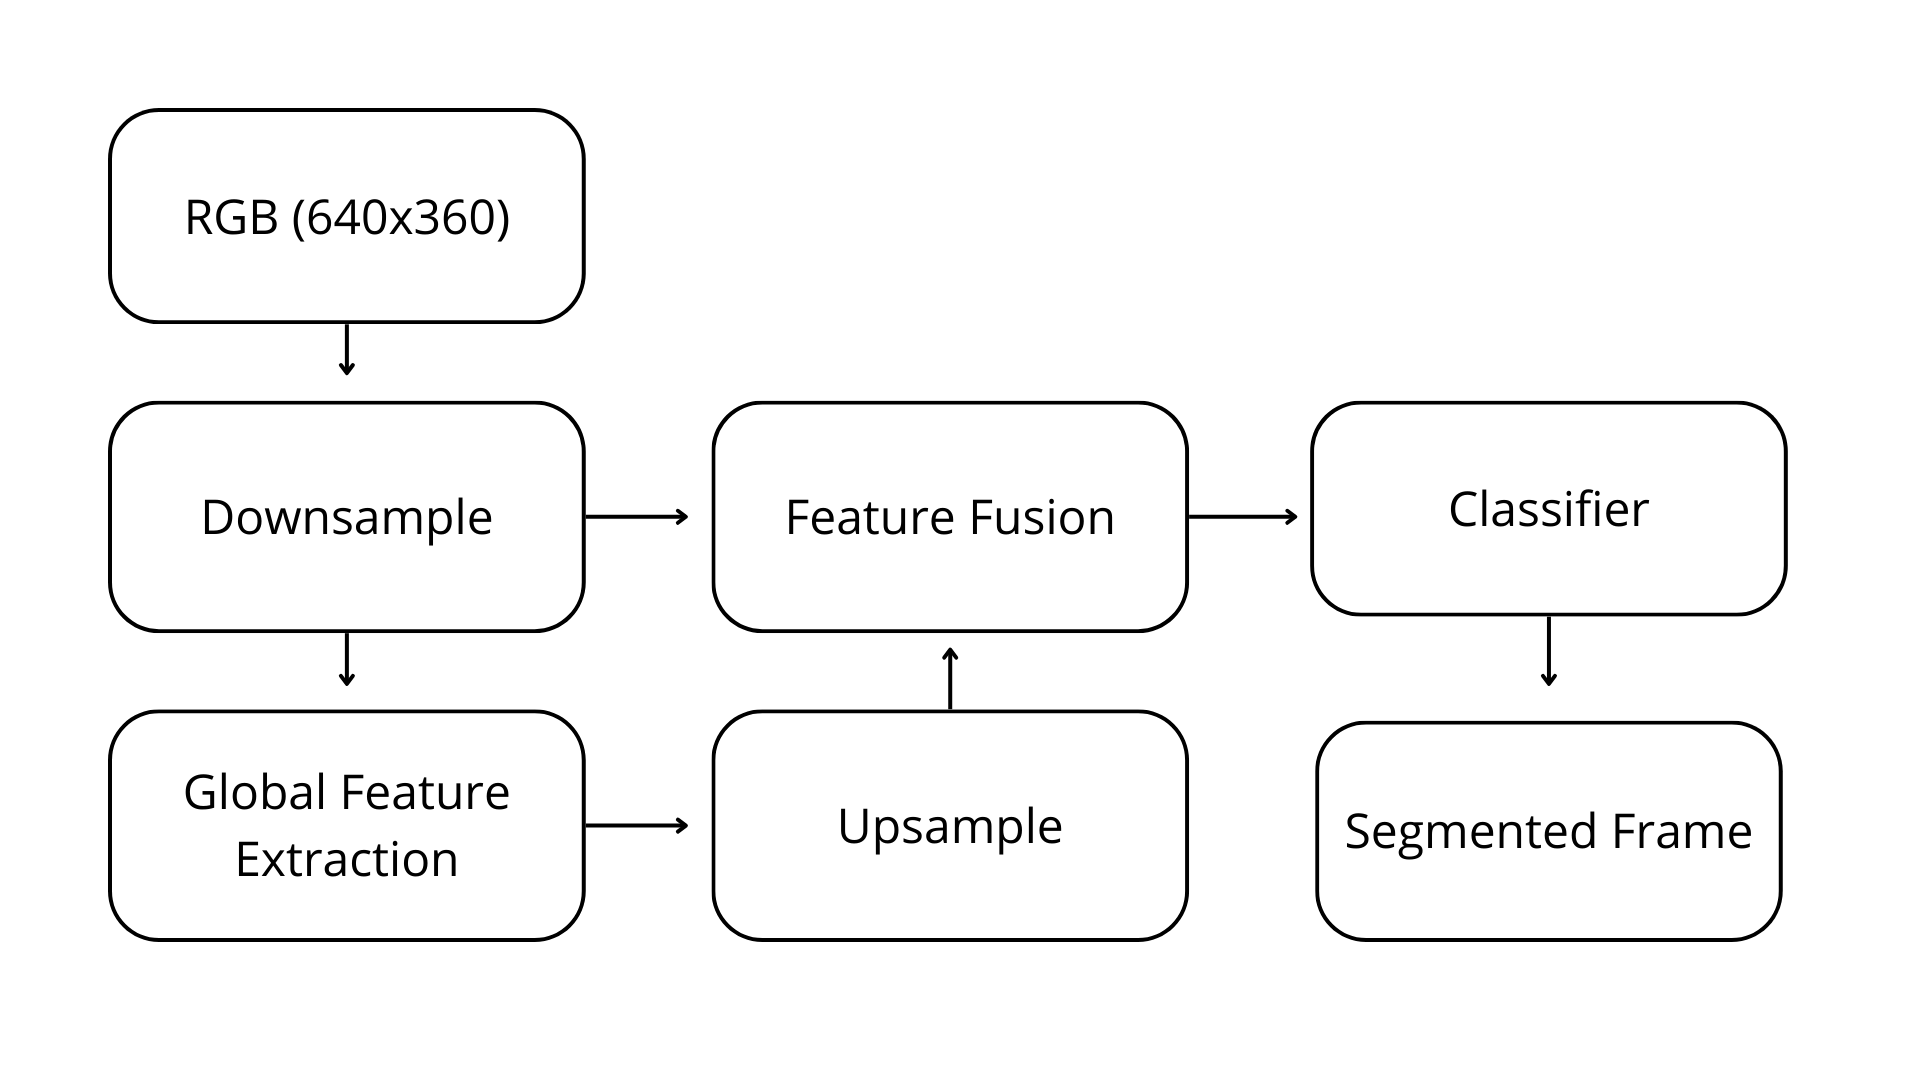
\includegraphics[width=\linewidth]{../konten/ml_sys.png}
	\caption{Block diagram of the Reduced Fast-SCNN architecture.}
	\label{fig:ml_system}
\end{figure}

Building upon the original Fast-SCNN architecture \cite{ref_fast_scnn}, we developed a modified version specifically optimized for lane detection in industrial settings. The original Fast-SCNN was designed for high-speed semantic segmentation on mobile devices; however, in our application, the focus is shifted from segmentation accuracy toward achieving real-time inference on limited computing hardware. The overall structure of the Reduced Fast-SCNN is shown in Fig.~\ref{fig:ml_system}.

\subsubsection{Downsampling}
The Reduced Fast-SCNN begins with a downsampling stage that reduces the input image to a fixed resolution of 360$\times$640 pixels (width $\times$ height). To further reduce computational complexity, the number of convolutional channels is decreased. While the original Fast-SCNN employs 64 channels after downsampling, our modified version uses only 32 channels. This reduction effectively lowers the processing load, with a marginal trade-off in segmentation precision—an acceptable compromise for static and structured industrial environments.

\subsubsection{Global Feature Extraction}
Following the same principle, the global feature extraction stage also reduces the number of channels. In the original architecture, this stage uses 128 channels, whereas in the Reduced Fast-SCNN it is limited to 64 channels. Additionally, the pyramid pooling module is replaced with a lightweight average pooling layer. Compared to pyramid pooling, average pooling simplifies the computation and improves inference speed, making it more suitable for CPU-only real-time operation.

\subsubsection{Upsampling, Feature Fusion, and Classification}
The upsampling, feature fusion, and classification stages retain the core structure of the original Fast-SCNN but operate with fewer convolutional channels. The final output of the Reduced Fast-SCNN is a binary segmentation mask representing two classes: lane and non-lane regions. This segmentation output is later utilized to compute a confidence level that influences the vehicle’s navigation decisions, particularly in adjusting steering and velocity control.

\subsection{Integration of Both Systems}
\begin{figure}[H]
	\centering
	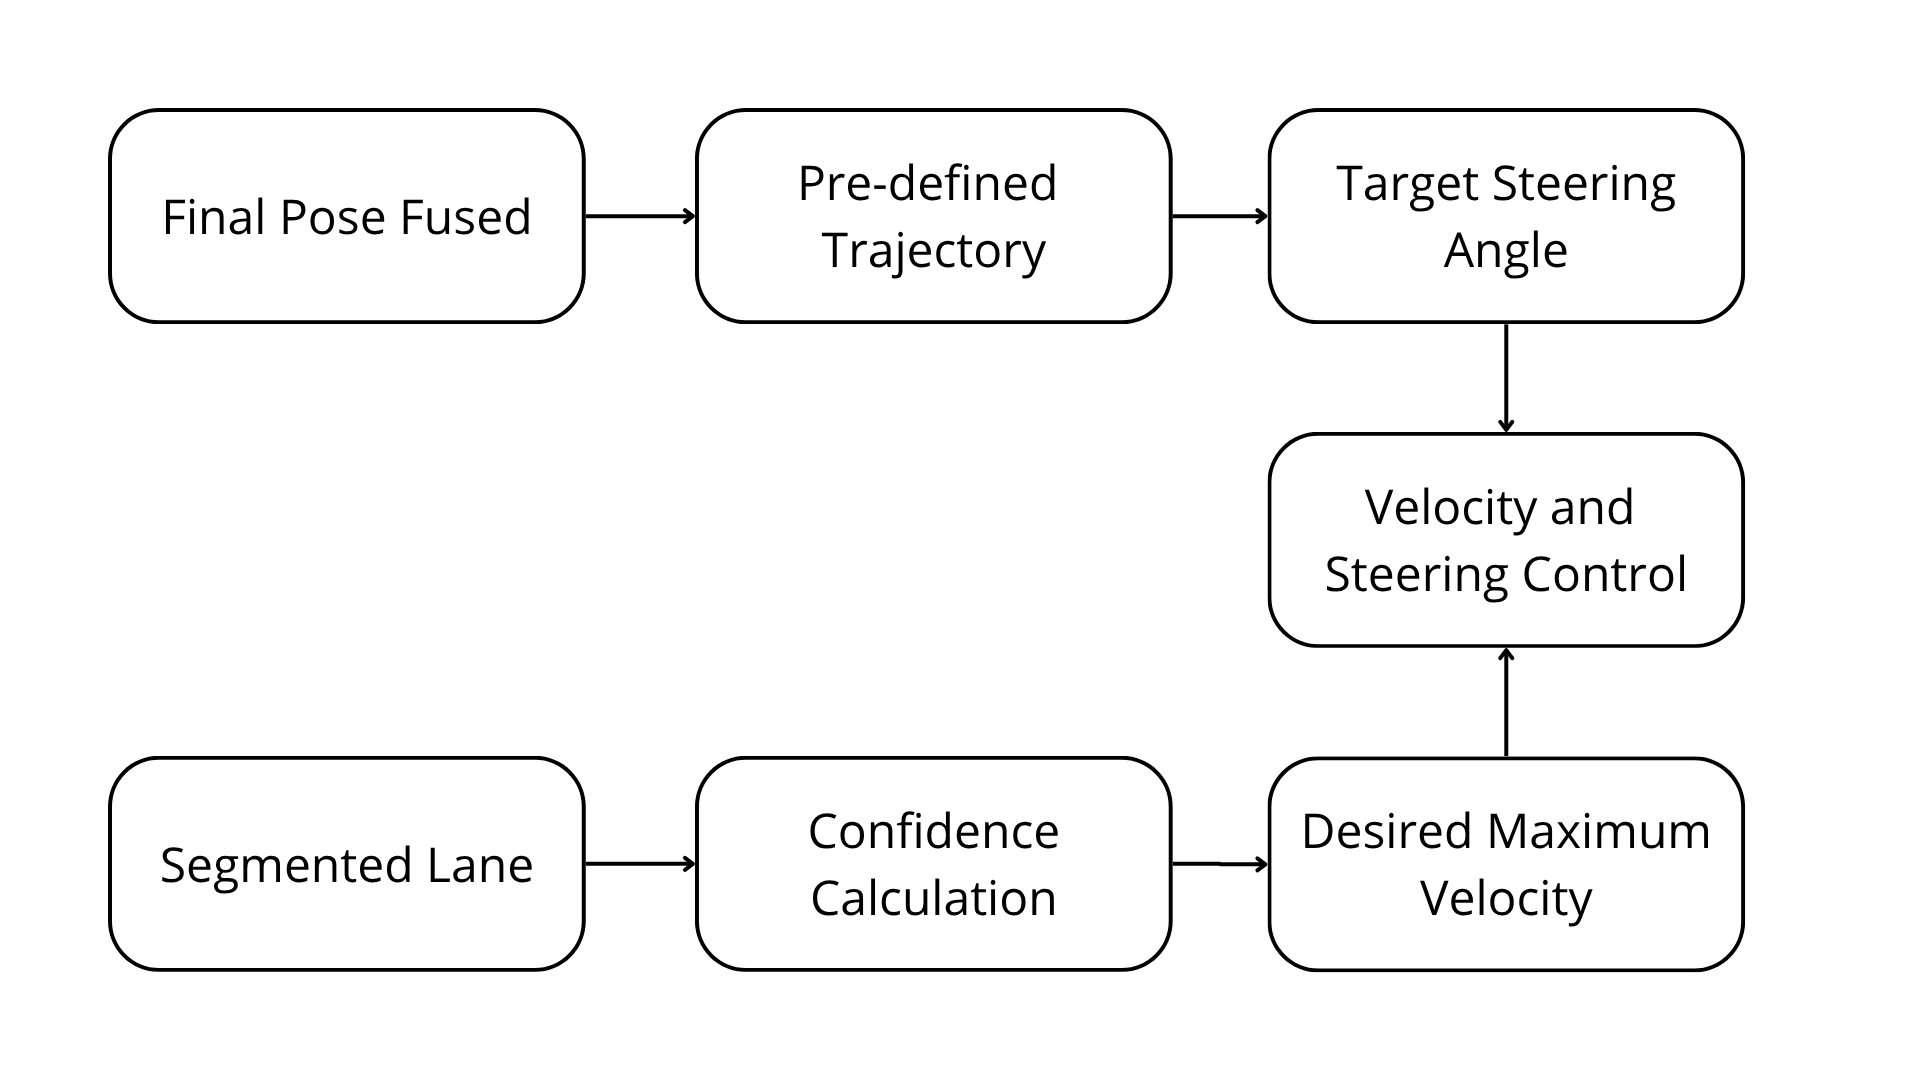
\includegraphics[width=\linewidth]{../konten/hahhhh.png}
	\caption{Integration of the Extended RTAB-Map and Reduced Fast-SCNN for the navigation system.}
	\label{fig:nav_new_system}
\end{figure}

Figure~\ref{fig:nav_new_system} presents the integrated architecture combining the Extended RTAB-Map for global localization and the Reduced Fast-SCNN for local perception. The navigation controller calculates the heading direction to the next waypoint as:

\begin{equation}
	\theta_{\text{direction}} = \tan^{-1}\!\left(\frac{y_{\text{wp}} - y_{\text{position}}}{x_{\text{wp}} - x_{\text{position}}}\right) - \theta_{\text{orientation}}
	\label{eq:waypoint_angle}
\end{equation}

where $x_{\text{wp}}$ and $y_{\text{wp}}$ are the coordinates of the next waypoint from the predefined trajectory, $x_{\text{position}}$ and $y_{\text{position}}$ represent the current vehicle position, and $\theta_{\text{orientation}}$ denotes the current vehicle heading. The resulting $\theta_{\text{direction}}$ is the desired heading angle toward the waypoint.

\par
Using the Bicycle Model \cite{rajamani2011vehicle}, the target steering angle is calculated as:

\begin{equation}
	\delta_{\text{target}} = \tan^{-1}\!\left( \frac{2L \sin(\theta_{\text{direction}})}{D_{\text{lookahead}}} \right)
	\label{eq:bicycle_model_full}
\end{equation}

where $L$ is the wheelbase (distance between front and rear axles), and $D_{\text{lookahead}}$ is the lookahead distance. The variable $\delta_{\text{target}}$ represents the desired steering angle for the vehicle.

\par
Next, the system computes a confidence level from the segmented lane detection image. This confidence represents the proportion of detected lane area relative to a predefined region of interest (ROI) and is calculated as:

\begin{equation}
	\text{normal} = \frac{\text{area of segmented lane detection}}{\text{area of ROI}}
	\label{eq:confidence_level}
\end{equation}

where the numerator denotes the pixel area of the detected lane, and the denominator corresponds to the ROI area. The resulting $\text{normal}$ value lies between 0 and 1.

\par
The confidence value is then used to determine the target speed according to:

\begin{equation}
	v_{\text{target\_max}} = v_{\text{max}} \cdot \text{normal}^2
	\label{eq:confidence_speed}
\end{equation}

where $v_{\text{max}}$ is the maximum allowed velocity of the vehicle, and $v_{\text{target\_max}}$ is the confidence-adjusted maximum speed. This ensures the vehicle moves more cautiously when lane confidence is low.

\par
To ensure smooth transitions and suppress sudden speed fluctuations caused by segmentation noise or image flickering, a first-order low-pass filter is applied:

\begin{equation}
	v_{\text{target}} = \alpha \cdot v_{\text{target\_max}} + (1 - \alpha) \cdot v_{\text{target}}
	\label{eq:low_pass_filter}
\end{equation}

where $\alpha$ is the smoothing coefficient (set to 0.055), $v_{\text{target\_max}}$ is the instantaneous target speed, and $v_{\text{target}}$ is the previously filtered speed. The final output, $v_{\text{target}}$, is used to control the vehicle’s longitudinal motion, while $\delta_{\text{target}}$ regulates steering. Both values are transmitted to the low-level control layer to execute the motion commands in real time.

\par
By combining these two subsystems, the navigation system achieves real-time perception and high-frequency localization, enabling stable and accurate motion control even on limited hardware resources.


\section{Results and Discussion}
\subsection{Hardware Odometry vs.\ Extended RTAB-Map}
Table~\ref{tab:pose_estimation} shows pose drift after a 500~m trajectory using odometry only; Table~\ref{tab:pose_estimation_slam} shows the extended method.

\begin{table}[H]
	\centering
	\caption{Pose Estimation Result: Hardware Odometry Only}
	\label{tab:pose_estimation}
	\begin{tabular}{|c|c|c|c|}
		\hline
		\textbf{Lap-} & \textbf{X (m)} & \textbf{Y (m)} & \textbf{Error (m)} \\ \hline
		1 & 0.28 & 0.39 & 0.48 \\ \hline
		2 & 0.30 & 0.43 & 0.52 \\ \hline
		3 & 0.24 & 0.49 & 0.55 \\ \hline
		4 & 0.18 & 0.32 & 0.37 \\ \hline
		5 & 0.37 & 0.41 & 0.55 \\ \hline
		\multicolumn{3}{|c|}{\textbf{Average Error}} & 0.494 \\ \hline
	\end{tabular}
\end{table}

\begin{table}[H]
	\centering
	\caption{Pose Estimation Result: Extended RTAB-Map}
	\label{tab:pose_estimation_slam}
	\begin{tabular}{|c|c|c|c|}
		\hline
		\textbf{Lap-} & \textbf{X (m)} & \textbf{Y (m)} & \textbf{Error (m)} \\ \hline
		1 & 0.01 & 0.02 & 0.02 \\ \hline
		2 & 0.00 & 0.03 & 0.03 \\ \hline
		3 & 0.01 & 0.02 & 0.02 \\ \hline
		4 & 0.02 & 0.01 & 0.02 \\ \hline
		5 & 0.04 & 0.01 & 0.04 \\ \hline
		\multicolumn{3}{|c|}{\textbf{Average Error}} & 0.026 \\ \hline
	\end{tabular}
\end{table}

Figures~\ref{fig:map_hw_odom} and \ref{fig:map_extended_rtabmap} visualize the difference in occupancy mapping relative to the ground-truth path (blue line).

\begin{figure}[H]
	\centering
	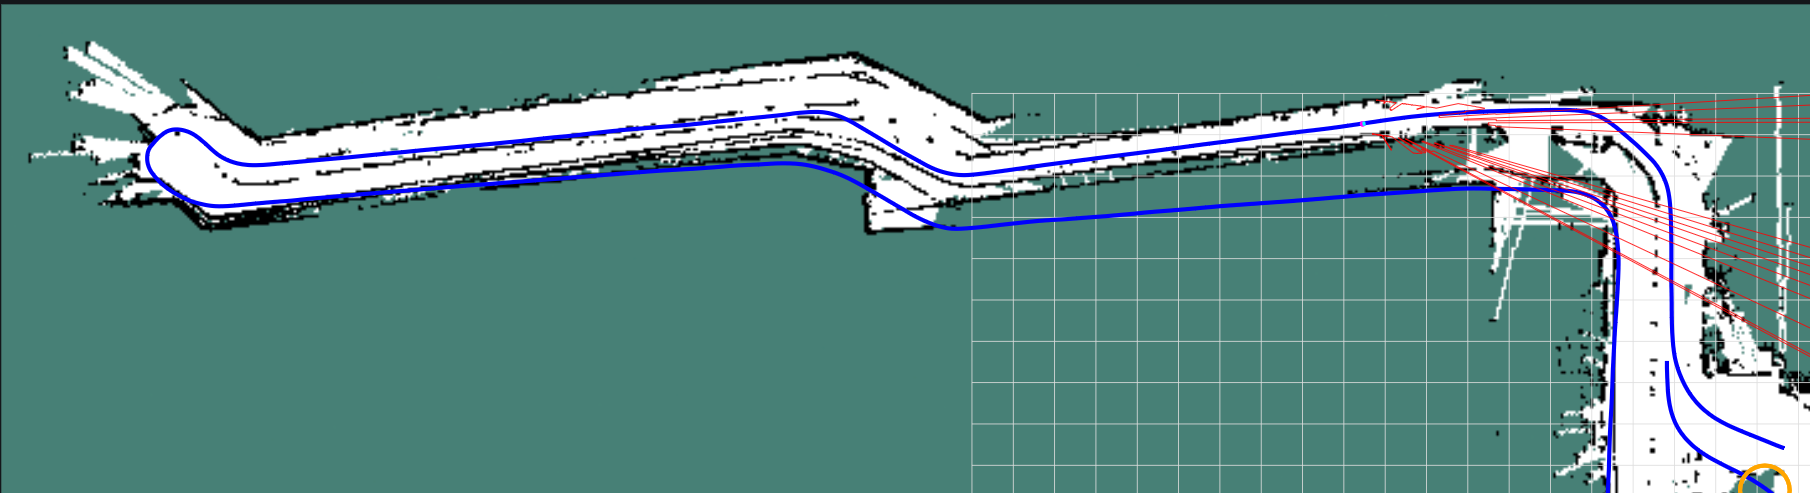
\includegraphics[width=\linewidth]{../konten/map_salah.png}
	\caption{Occupancy grid map using hardware odometry only.}
	\label{fig:map_hw_odom}
\end{figure}

\begin{figure}[H]
	\centering
	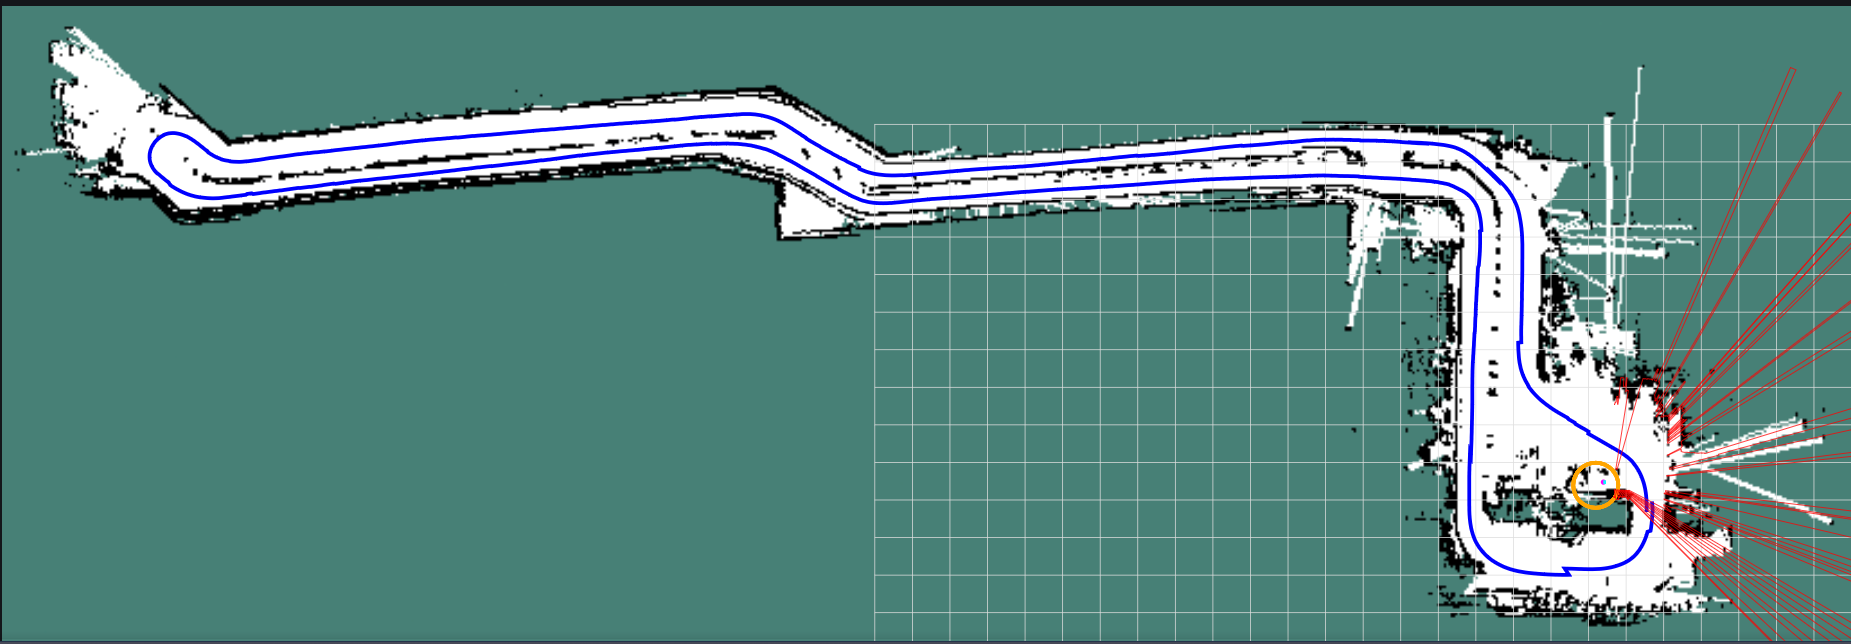
\includegraphics[width=\linewidth]{../konten/map_benar.png}
	\caption{Occupancy grid map using Extended RTAB-Map.}
	\label{fig:map_extended_rtabmap}
\end{figure}

\subsection{Update Rate: Default vs.\ Extended RTAB-Map}
Update rates were measured via ROS topic frequency tools (Table~\ref{tab:update_rate}). The extended method delivers $\sim$50~Hz fused pose.

\begin{table}[H]
	\centering
	\caption{Update Rate: Default RTAB-Map vs.\ Extended RTAB-Map}
	\label{tab:update_rate}
	\begin{tabular}{|c|c|c|}
		\hline
		\textbf{Lap-} & \textbf{RTAB-Map (Hz)} & \textbf{Extended RTAB-Map (Hz)}  \\ \hline
		1 & 1.003 & 50.029 \\ \hline
		2 & 1.002 & 50.006 \\ \hline
		3 & 1.223 & 49.999 \\ \hline
		4 & 1.056 & 49.999 \\ \hline
		5 & 1.332 & 49.998 \\ \hline
		\textbf{Average} & 1.123 & 50.006 \\ \hline
	\end{tabular}
\end{table}

\subsection{Reduced Fast-SCNN Results}
The Reduced Fast-SCNN was trained on a custom dataset of 797 images (size $640\times360\times3$). The dataset was used in full for training due to its domain specificity. Training used Adam (lr $=10^{-4}$), batch size 4, for 100 epochs. Sample images are shown in Fig.~\ref{fig:dataset_sample}.

\begin{figure}[H]
	\centering
	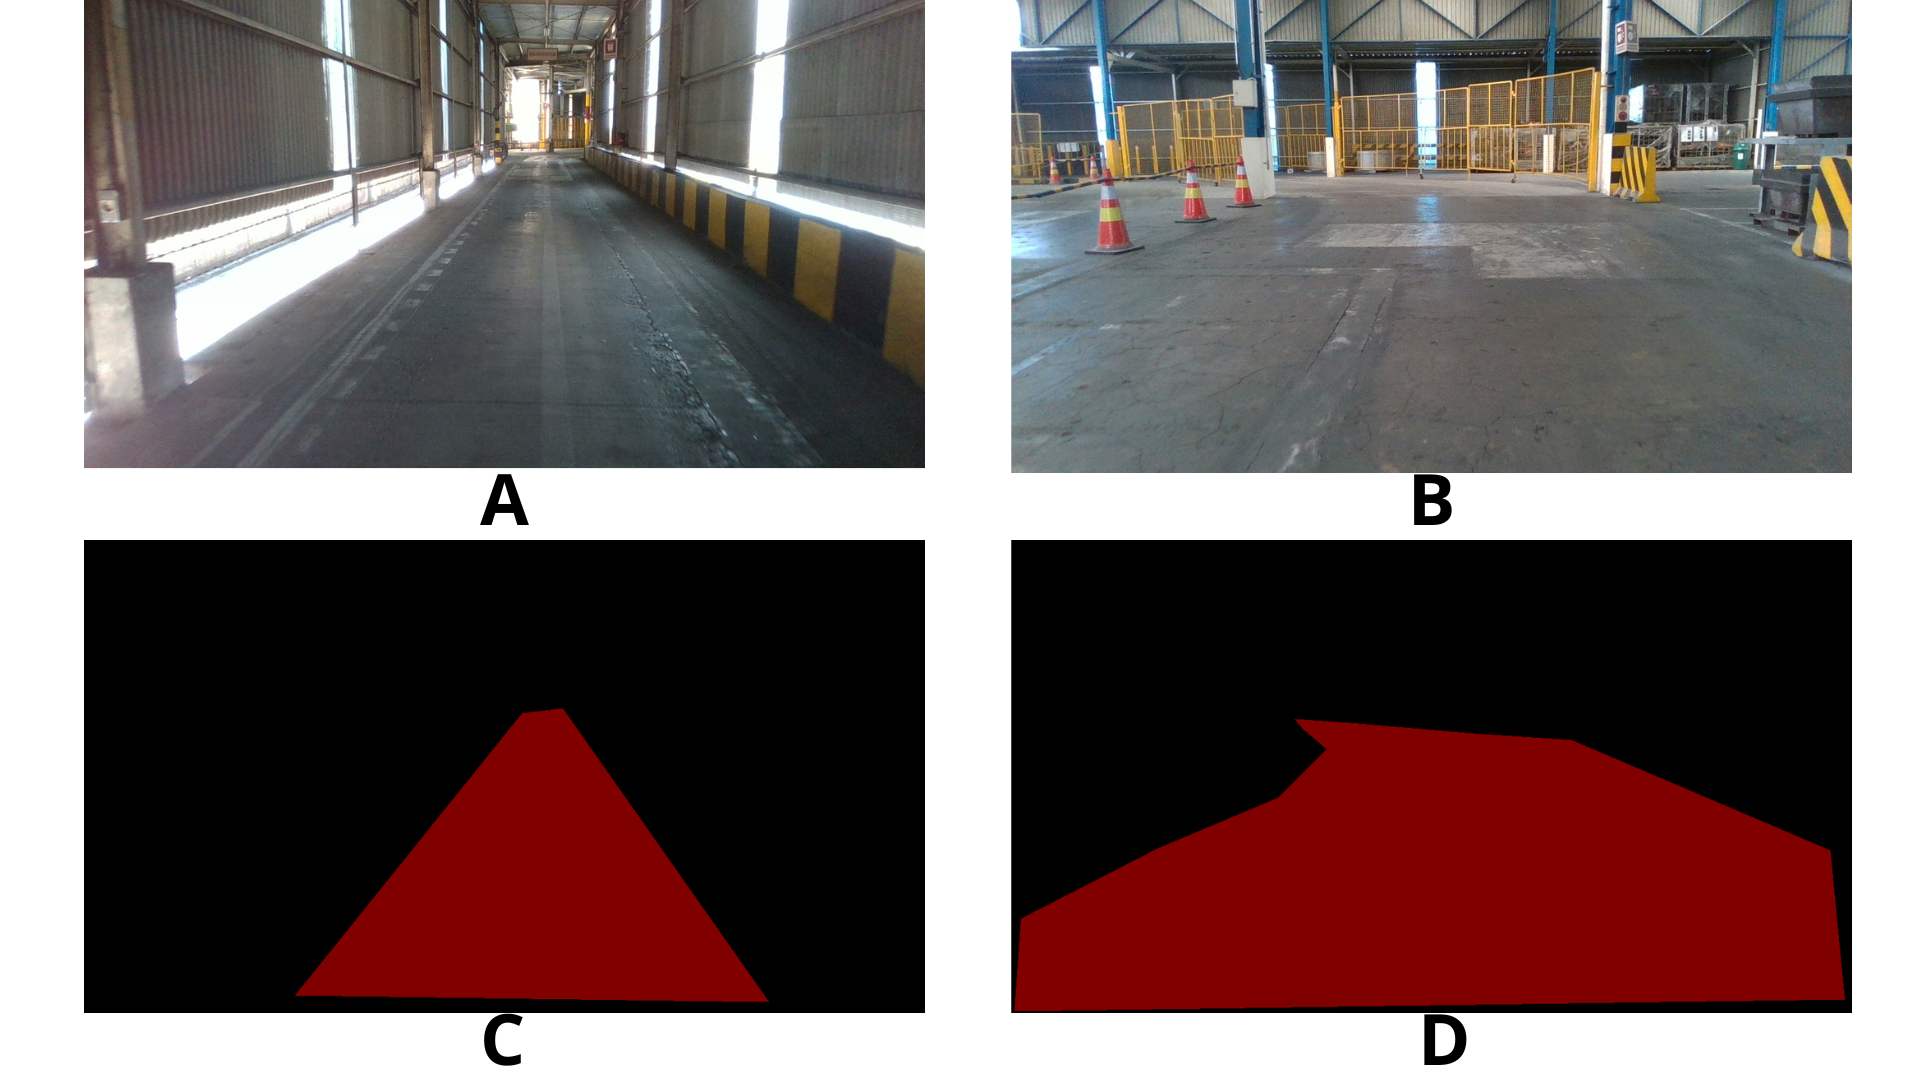
\includegraphics[width=\linewidth]{../konten/dataset_ist.png}
	\caption{Sample of the custom dataset (RGB inputs and lane masks).}
	\label{fig:dataset_sample}
\end{figure}

After training, the model was exported to ONNX. Using ONNX Runtime provided $\sim\!2\times$ faster inference \cite{ref_onnx}. Pre-results for lane detection with an ROI overlay are shown in Fig.~\ref{fig:roi_lane_detection}.

\begin{figure}[H]
	\centering
	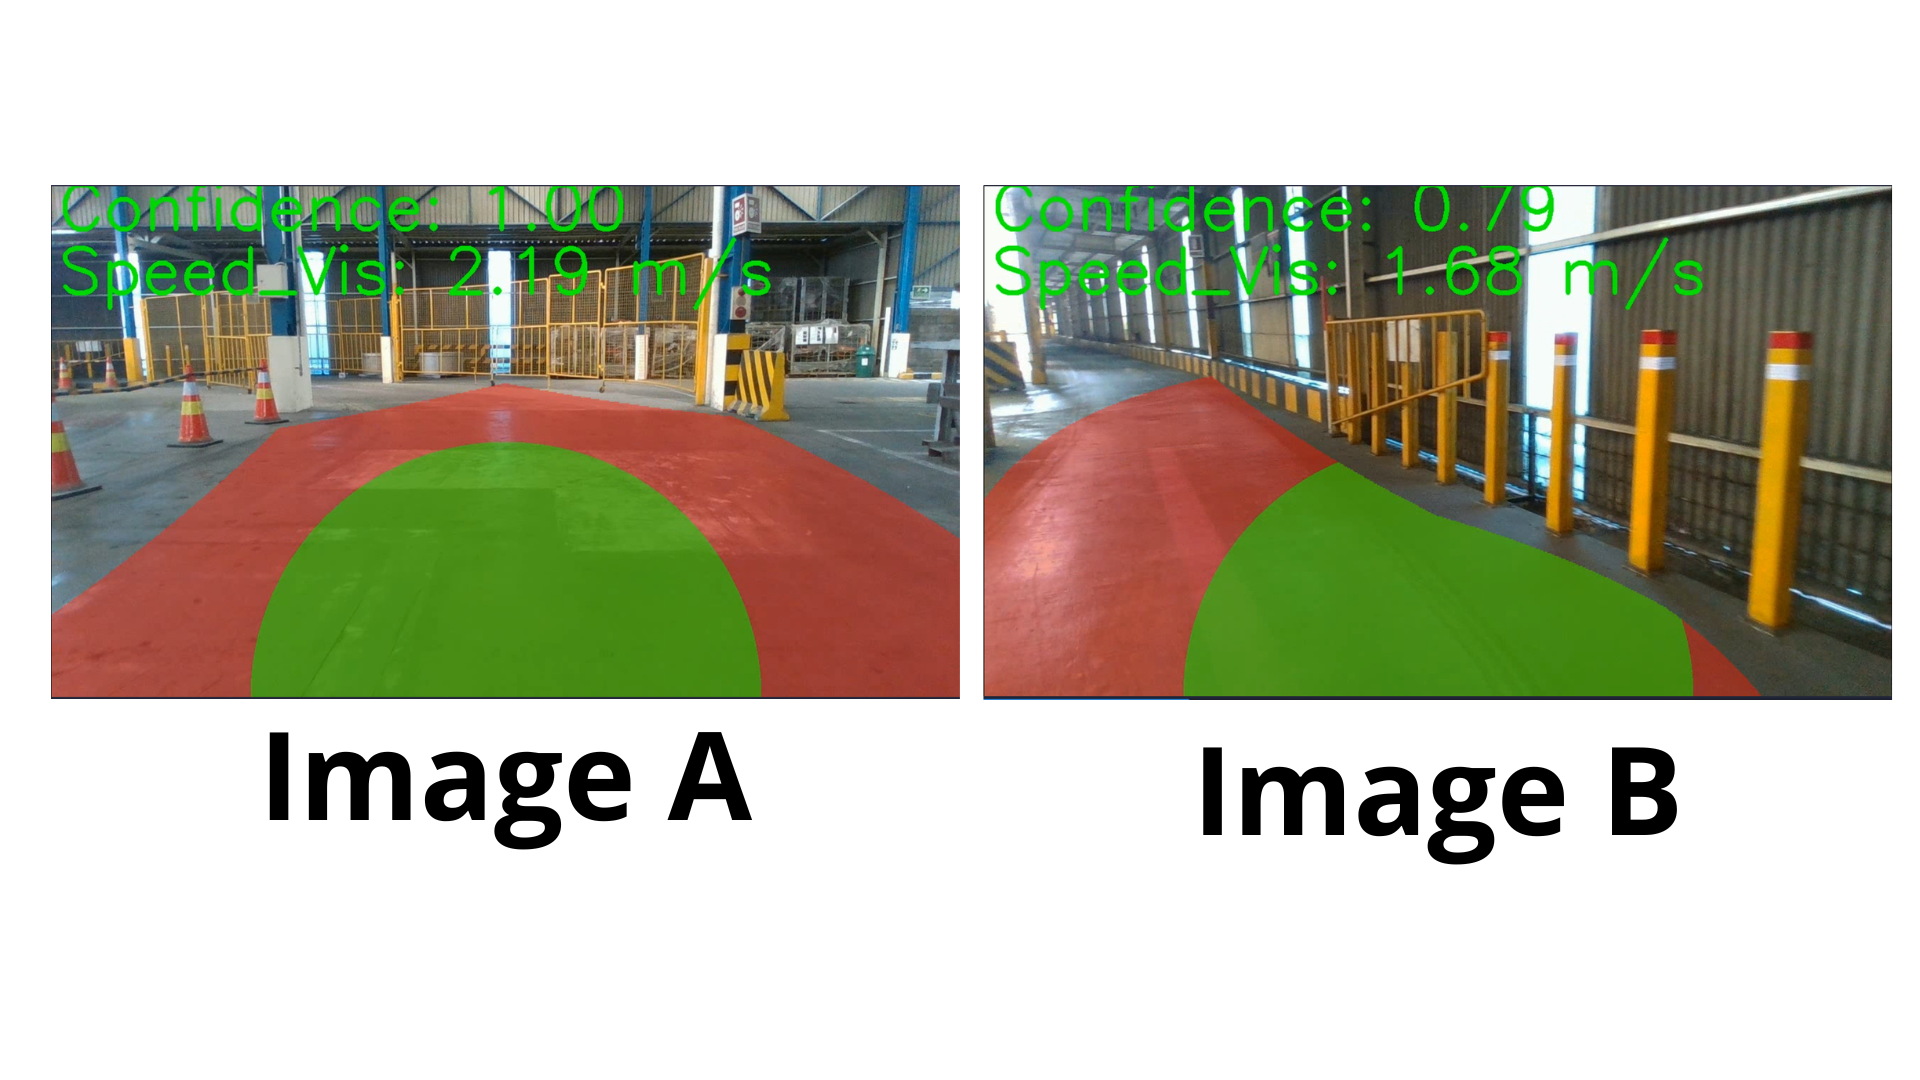
\includegraphics[width=\linewidth]{../konten/pre_res.png}
	\caption{ROI-based lane detection using the Reduced Fast-SCNN.}
	\label{fig:roi_lane_detection}
\end{figure}

Representative outcomes and corresponding velocities are shown in Fig.~\ref{fig:lane_detection_result}: (A) full straight lane ($v\!=\!2.2$~m/s), (B) narrow straight lane ($v\!=\!1.76$~m/s), (C) sharp turn facing fences ($v\!=\!0.70$~m/s), (D) approaching left turn in a narrow area ($v\!=\!1.59$~m/s), (E) obstacle ahead (stop, $v\!=\!0$), (F) right turn in a narrow area ($v\!=\!1.56$~m/s).

\begin{figure}[H]
	\centering
	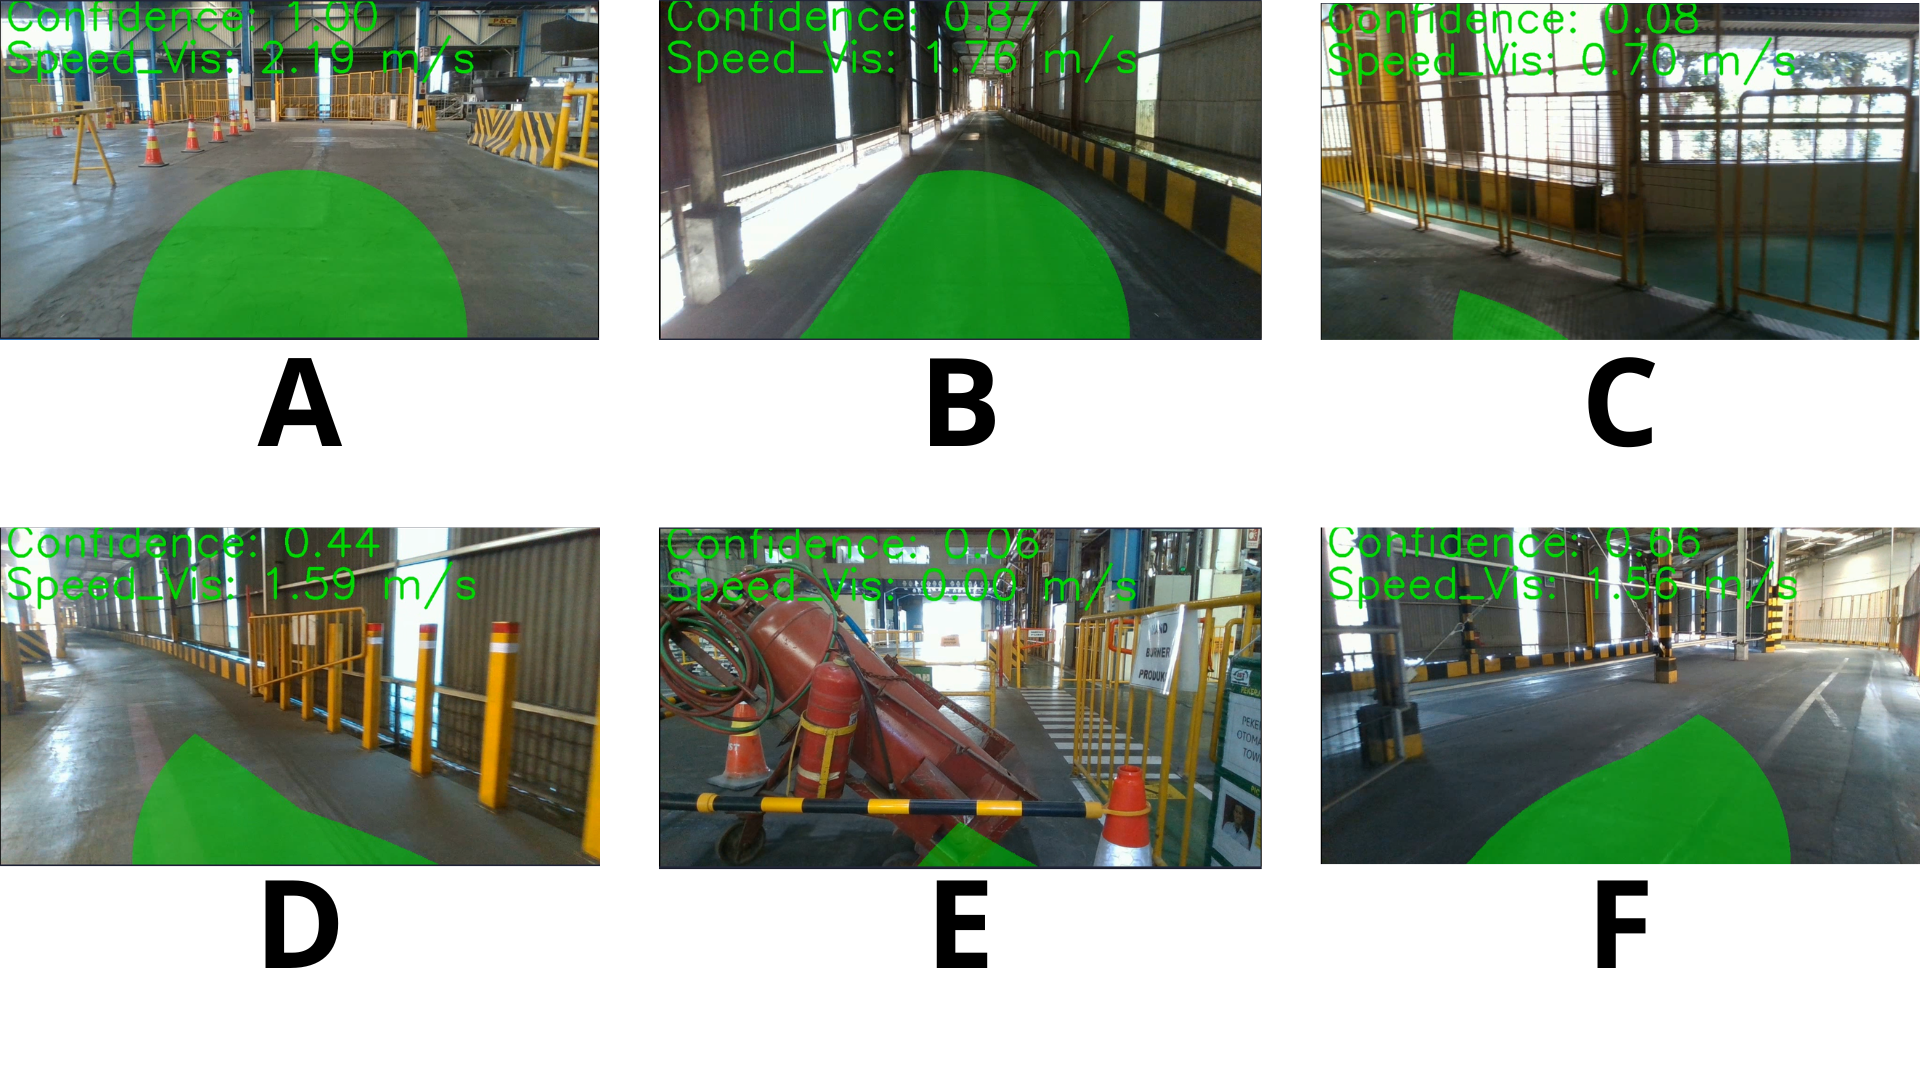
\includegraphics[width=\linewidth]{../konten/bnr_satu.png}
	\caption{Lane detection results and resulting target velocities.}
	\label{fig:lane_detection_result}
\end{figure}

\subsection{Inference Time: Original vs.\ Reduced Fast-SCNN}
Inference was benchmarked on an Intel i5 12th Gen CPU with 16~GB RAM and Intel Iris Xe Graphics, using identical $640\times360\times3$ images (Table~\ref{tab:lane_detection_inference_time}).

\begin{table}[H]
	\centering
	\caption{Inference Time: Original vs.\ Reduced Fast-SCNN}
	\label{tab:lane_detection_inference_time}
	\begin{tabular}{|c|c|c|}
		\hline
		\textbf{Frame Number} & \textbf{Fast-SCNN (ms)} & \textbf{Reduced Fast-SCNN (ms)} \\ \hline
		1 & 22.4 & 7.2 \\ \hline
		2 & 29.3 & 7.7 \\ \hline
		3 & 34.2 & 7.8 \\ \hline
		4 & 39.2 & 7.7 \\ \hline
		5 & 23.8 & 7.4 \\ \hline
		6 & 28.1 & 8.0 \\ \hline
		\textbf{Average} & 29.5 & 7.63 \\ \hline
	\end{tabular}
\end{table}

On average, the Reduced Fast-SCNN is $\sim$3.9$\times$ faster (7.63~ms vs.\ 29.5~ms), enabling CPU-only real-time operation.

\section{Future Development}
Future work includes: (1) improving robustness by adding temporal context via GRU-based modules \cite{ref_gru}, and (2) learning velocity and steering directly from perception and pose through end-to-end ML.

\section{Conclusion}
By augmenting RTAB-Map with hardware odometry and Kalman fusion, we achieve centimeter-level pose accuracy with a 50~Hz update rate on a CPU-only platform. The Reduced Fast-SCNN attains sub-10~ms inference, making the combined navigation stack efficient and suitable for industrial autonomous vehicles.

\section{Acknowledgment}
This work was supported by Indonesia Smelting Technology (IST), Manufaktur Robot Industri (MRI), and ITS Robotics. The authors thank the supporting teams for their assistance. We also acknowledge ChatGPT and GitHub Copilot for writing support.

\bibliographystyle{IEEEtranN}
\bibliography{../ubah/pustaka.bib}

% \balance  % Uncomment if you need balanced columns on the last page
\end{document}
